\documentclass[12pt]{article}
\usepackage{lecture}
\usepackage{html}
\usepackage{url}
\usepackage{graphicx}

\newcommand{\copyrightYears}{2001-2023}

\title{Analyzing the genetic structure of populations}

\begin{document}

\maketitle

\thispagestyle{first}

\section*{Introduction}

So far we've focused on inbreeding as one important way that
populations may fail to mate at random, but there's another way in
which virtually all populations and species fail to mate at
random. Individuals tend to mate with those that are nearby. Even
within a fairly small area, phenomena like nearest neighbor
pollination in flowering plants or home-site fidelity in animals can
cause mates to be selected in a geographically non-random way. What
are the population genetic consequences of this form of non-random
mating?\index{geographic structure}

Well, if you think about it a little, you can probably figure it
out. Since individuals that occur close to one another tend to be more
genetically similar than those that occur far apart, the impacts of
local mating will mimic those of inbreeding within a single,
well-mixed population.

\section*{A numerical example}

For example, suppose we have two subpopulations of green lacewings,
one of which occurs in forests the other of which occurs in adjacent
meadows.\footnote{Those of you who've been in EEB for a while will
  know that these are probably different species, but humor me, and
  forget that you know that.} Suppose further that within each
subpopulation mating occurs completely at random, but that there is no
mating between forest and meadow individuals. Suppose we've determined
allele frequencies in each population at a locus coding for
phosphoglucoisomerase ($PGI$), which conveniently has only two
alleles. The frequency of $A_1$ in the forest is 0.4 and in the meadow
in 0.7. We can easily calculate the expected genotype frequencies
within each population, namely\index{Wahlund effect}

\begin{center}
\begin{tabular}{l|rrr}
\hline\hline
       & $A_1A_1$ & $A_1A_2$ & $A_2A_2$ \\
\hline
Forest &     0.16 &     0.48 &     0.36 \\
Meadow &     0.49 &     0.42 &     0.09 \\
\hline
\end{tabular}
\end{center}

Suppose, however, we were to consider a combined population consisting
of 100 individuals from the forest subpopulation and 100 individuals
from the meadow subpopulation. Then we'd get the
following:\footnote{If we ignore sampling error.}

\begin{center}
\begin{tabular}{l|rrr}
\hline\hline
       & $A_1A_1$ & $A_1A_2$ & $A_2A_2$ \\
\hline
From forest & 16  & 48       & 36 \\
From meadow & 49  & 42       & 9 \\
\hline
Total       & 65  & 90       & 45 \\
\hline
\end{tabular}
\end{center}
So the frequency of $A_1$ is $(2(65) + 90)/(2(65 + 90 + 45)) =
0.55$. Notice that this is just the average allele frequency in the
two subpopulations, i.e., $(0.4 + 0.7)/2$. Since each subpopulation has
genotypes in Hardy-Weinberg proportions, you might expect the combined
population to have genotypes in Hardy-Weinberg proportions, but if you did
you'd be wrong. Just look.

\begin{center}
\begin{tabular}{l|rrr}
\hline\hline
                            & $A_1A_1$ & $A_1A_2$ & $A_2A_2$ \\
\hline
Expected (from $p=0.55$)    & (0.3025)200 & (0.4950)200 & (0.2025)200 \\
                            & 60.5     & 99.0     & 40.5 \\
Observed (from table above) & 65       & 90       & 45 \\
\hline
\end{tabular}
\end{center}
The expected and observed don't match, even though there is random
mating within both subpopulations. They don't match because there
isn't random mating {\it in the combined population}, only within each
subpopulation. Forest lacewings choose mates at random from other
forest lacewings, but they never mate with a meadow lacewing (and {\it
  vice versa\/}). Our sample includes two populations that don't
mix. As a result, heterozygotes in our combined sample are less
frequent ($0.45$ vs $0.495$) than we'd expect if the population were
well mixed with an allelel frequency of $0.55$. This is an example of
what's known as the {\it Wahlund effect}~\cite{Wahlund-1928}.\index{Wahlund effect}

\section*{The algebraic development}

Even though you've only known me for a couple of weeks now, you should
know me well enough to know that I'm not going to be satisfied with a
numerical example. You should know that I now feel the need to do some
algebra to describe this situation a little more generally.

Suppose we know allele frequencies in $k$ subpopulations.\footnote{For
  the time being, I'm going to assume that we know the allele
  frequencies without error, i.e., that we didn't have to estimate
  them from data. We'll deal with real life, i.e., how we can detect
  the Wahlund effect when we have to {\it estimate\/} allele
  freqeuncies from data, a little later.} Let $p_i$ be the frequency
of $A_1$ in the $i$th subpopulation. Then if we assume that all
subpopulations contribute equally to combined
population,\footnote{We'd get the same result by relaxing this
  assumption, but the algebra gets messier, so why bother?} we can
calculate expected and observed genotype frequencies the way we did
above:\index{Wahlund effect!theory}

\begin{center}
\begin{tabular}{l|rrr}
\hline\hline
         & $A_1A_1$       & $A_1A_2$         & $A_2A_2$ \\
\hline
Expected & $\bar p^2$     & $2\bar p\bar q$  & $\bar q^2$ \\
Observed & $\frack\sum p_i^2$ & $\frack\sum 2p_iq_i$ & $\frack\sum q_i^2$ \\
\hline
\end{tabular}
\end{center}
where $\bar p = \sum p_i/k$ and $\bar q = 1 - \bar p$ are the average
allele frequencies in the combined sample. Now
\begin{eqnarray}
\frack\sum p_i^2 &=& \frack\sum (p_i - \bar p + \bar p)^2 \\
&=& \frack\sum \left((p_i - \bar p)^2 + 2\bar p(p_i - \bar p)
                            + \bar p^2\right) \\
             &=& \frack\sum (p_i - \bar p)^2 + \bar p^2 \\
             &=& \hbox{Var}(p) + \bar p^2 \label{eq:p2}
\end{eqnarray}
Similarly,
\begin{eqnarray}
\frack\sum 2p_iq_i &=& 2\bar p\bar q - 2\hbox{Var}(p) \label{eq:2pq} \\
\frack\sum q_i^2   &=& \bar q^2 + \hbox{Var}(p) \label{eq:q2}
\end{eqnarray}

Since $\hbox{Var}(p) \ge 0$ by definition, with equality holding only
when all subpopulations have the same allele frequency, we can
conclude that\index{Wahlund effect!properties}

\begin{itemize}

\item Homozygotes will be more frequent and heterozygotes will be less
  frequent than expected based on the allele frequency in the combined
  population.

\item The magnitude of the departure from expectations is directly
  related to the magnitude of the variance in allele frequencies
  across populations, $\hbox{Var}(p)$.

\item The effect will apply to {\it any\/} mixing of samples in which
  the subpopulations combined have different allele
  frequencies.\footnote{For example, if we combine samples from
    different years or across age classes of long-lived organisms, we
    may see a deficienty of heterozygotes in the sample purely as a
    result of allele frequency differences across years. Remember that
    I told you one of the assumptions underlying derivation of the
    Hardy-Weinberg principle is that generations are
    non-overlapping? This is why.}

\item The same general phenomenon will occur if there are multiple
  alleles at a locus, although it is possible for one or a few
  heterozygotes to be {\it more\/} frequent than expected if there is
  positive covariance in the constituent allele frequencies across
  populations.\footnote{If you're curious about this, feel free to
    ask, but I'll have to dig out my copy of Li~\cite{Li-1976} to
    answer. I don't carry those details around in my head.}

\item The effect is analogous to inbreeding. Homozygotes are more
  frequent and heterozygotes are less frequent than
  expected.\footnote{And this is what we predicted when we started.}

\end{itemize}

To return to our earlier numerical example:

\begin{eqnarray}
\hbox{Var}(p) &=& \left((0.4 - 0.55)^2 + (0.7 - 0.55)^2\right)/2 \\
              &=& 0.0225
\end{eqnarray}
\begin{center}
\begin{tabular}{l|rcrcr}
\hline\hline
         & Expected &   &           &   & Observed \\
\hline
$A_1A_1$ &   0.3025 & + &   0.0225  & = &   0.3250 \\
$A_1A_2$ &   0.4950 & - & 2(0.0225) & = &   0.4500 \\
$A_2A_2$ &   0.2025 & + &   0.0225  & = &   0.2250 \\
\hline
\end{tabular}
\end{center}

\section*{Wright's $F$-statistics}\index{F-statistics@$F$-statistics}

One limitation of the way I've described things so far is that
$\hbox{Var}(p)$ doesn't provide a convenient way to compare population
structure from different samples. $\hbox{Var}(p)$ can be much larger
if both alleles are about equally common in the whole sample than if
one occurs at a mean frequency of 0.99 and the other at a frequency of
0.01. Moreover, if you stare at equations (\ref{eq:p2})--(\ref{eq:q2})
for a while, you begin to realize that they look a lot like some
equations we've already encountered. Namely, if we were to define
$F_{st}$\footnote{The reason for the subscript will become apparent
  later. It's also {\it very\/} important to notice that I'm defining
  $F_{ST}$ here in terms of the population parameters $p$ and
  $\mbox{Var}(p)$. Again, we'll return to the problem of how to {\it
    estimate\/} $F_{ST}$ from data a little later.} as
$\mbox{Var}(p)/\bar p\bar q$, then we could rewrite equations
(\ref{eq:p2})--(\ref{eq:q2}) as
\begin{eqnarray}
\frack\sum p_i^2 &=& \bar p^2 + F_{st}\bar p \bar q \label{eq:p2-f} \\
\frack\sum 2p_iq_i &=& 2\bar p\bar q(1 - F_{st}) \label{eq:2pq-f} \\
\frack\sum q_i^2   &=& \bar q^2 + F_{st}\bar p \bar q \label{eq:q2-f}
\end{eqnarray}
And it's not even completely artificial to define $F_{st}$ the way I
did. After all, the effect of geographic structure is to cause matings
to occur among genetically similar individuals. It's rather like
inbreeding.\footnote{To be precise, it is a form of positive
  assortative mating in which the choice of mates is based on
  geographical proximity.}  Moreover, the extent to which this local
mating matters depends on the extent to which populations differ from
one another. It turns out that $\bar p\bar q$ is the maximum allele
frequency variance possible, given the observed mean frequency. So one
way of thinking about $F_{st}$ is that it measures the amount of
allele frequency variance in a sample relative to the maximum
possible.\footnote{I say ``one way'', because there are several other
  ways to talk about $F_{st}$, too. But we won't talk about them until
  later.}

There may, of course, be inbreeding within populations, too. But it's
easy to incorporate this into the framework, too.\footnote{At least
  it's easy once you've been shown how.} Let $H_i$ be the actual
heterozygosity in individuals within subpopulations, $H_s$ be the
expected heterozygosity within subpopulations assuming Hardy-Weinberg
within populations, and $H_t$ be the expected heterozygosity in the
combined population assuming Hardy-Weinberg over the whole
sample.\footnote{Please remember that we're assuming we know those
  frequencies exactly. In real applications, of course, we'll {\it
    estimate\/} those frequencies from data, so we'll have to account
  for sampling error when we actually try to estimate these things. If
  you're getting the impression that I think the distinction between
  allele frequencies as {\it parameters\/}, i.e., the real allele
  frequency in the population , and allele frequencies as {\it
    estimates\/}, i.e., the sample frequencies from which we hope to
  estimate the paramters, is really important, you're getting the
  right impression.}  Then thinking of $f$ as a measure of departure
from Hardy-Weinberg and assuming that all populations depart from
Hardy-Weinberg to the same degree, i.e., that they all have the same
$f$, we can define
\[
F_{it} = 1 - \frac{H_i}{H_t} \quad .
\]
$F_{it}$ is the overall departure from Hardy-Weinberg in the entire
sample. Let's fiddle with $F_{ST}$ a bit.\footnote{Are you beginning
  to see how peculiar I am? Do you know anyone else who gets a kick
  out of playing around with formulas and equations.}
\begin{eqnarray*}
1 - F_{it} &=& \frac{H_i}{H_t} \\
           &=& \left(\frac{H_i}{H_s}\right)\left(\frac{H_s}{H_t}\right) \\
           &=& (1 - F_{is})(1 - F_{st}) \quad ,
\end{eqnarray*}
where $F_{is}$ is the inbreeding coefficient within populations, i.e.,
$f$, and $F_{st}$ has the same definition as before.\footnote{It takes
  a fair amount of algebra to show that this definition of $F_{st}$ is
  equivalent to the one I showed you before, so you'll just have to
  take my word for it.} $H_t$ is often referred to as the genetic
diversity in a population. So another way of thinking about $F_{st} =
(H_t - H_s)/H_t$ is that it's the proportion of the diversity in the
sample that's due to allele frequency differences among populations.

\section*{Estimating $F$-statistics}

We've now seen the principles underlying Wright's $F$-statistics. I
should point out that Gustave Mal{\'e}cot developed very similar ideas
at about the same time as Wright, but since Wright's notation
stuck,\footnote{Probably because he published in English and
  Mal{\'e}cot published in French.} population geneticists generally
refer to statistics like those we've discussed as Wright's
$F$-statistics.\footnote{The Hardy-Weinberg proportions should
  probably be referred to as the Hardy-Weinberg-Castle proportions
  too, since Castle pointed out the same principle. For some reason,
  though, his demonstration didn't have the impact that Hardy's and
  Weinberg's did. So we generally talk about the Hardy-Weinberg
  principle.}

Neither Wright nor Mal{\'e}cot worried too much about the problem of
estimating $F$-statistics from data. Both realized that any inferences
about population structure are based on a sample and that the
characteristics of the sample may differ from those of the population
from which it was drawn, but neither developed any explicit way of
dealing with those differences. Wright develops some very {\it ad
  hoc\/} approaches in his book~\cite{Wright69}, but they have been
forgotten, which is good because they aren't satisfactory and they
shouldn't be used. There are now three reasonable approaches
available:\index{F-statistics@$F$-statistics}\footnote{And as we'll
  soon see, I'm not too crazy about one of these three. To my mind,
  there are really only two approaches that anyone should consider,
  and those two approaches are really just variants of the same basic
  idea.}

\begin{enumerate}

\item Nei's $G$-statistics,

\item Weir and Cockerham's $\theta$-statistics, and

\item A Bayesian analog of $\theta$.\footnote{This is, as you have
    probably already guessed, my personal favorite. We don't have time
    to discuss it in lecture, but if you're interested, ask me about
    it. I should also tell you that Gregory Owens pointed out on
    Twitter that arguments about genetic differentiation can get a
    little heated
    (\url{https://twitter.com/Greg_Owens/status/1582104811629346817}). They
    may not turn into an actual fistfight, but there have been some
    pretty extreme statements made.
  \begin{center}
    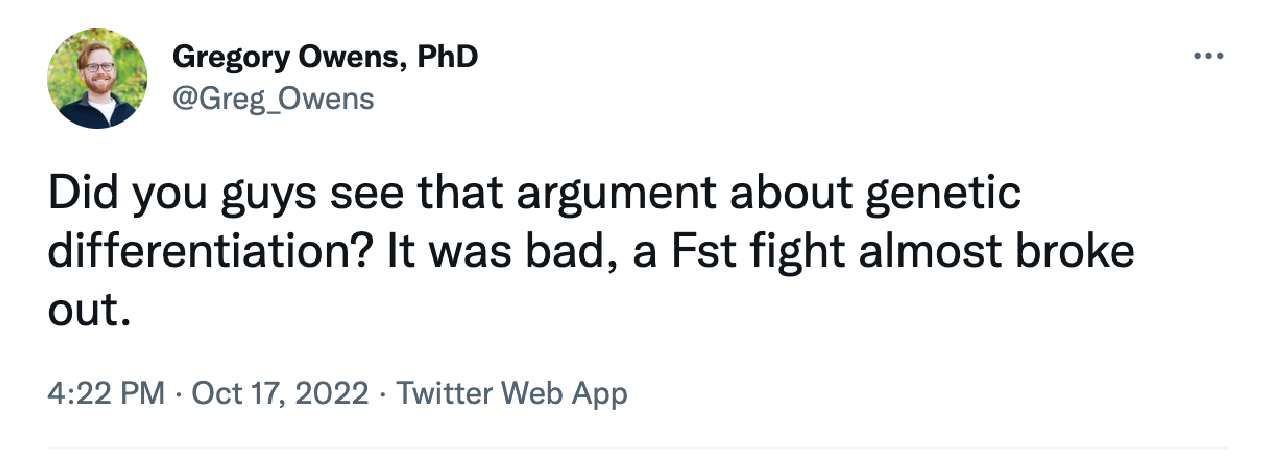
\includegraphics[height=2.5cm]{Fst-fight.eps}
  \end{center}}

\end{enumerate}

\section*{An example from {\it Isotoma petraea}}

To make the differences in implementation and calculation clear, I'm
going to use data from 12 populations of {\it Isotoma petraea\/} in
southwestern Australia surveyed for genotype at {\it
  GOT\/}--1~\cite{James-etal-1983} as an example throughout these
discussions~(Table~\ref{table:isotoma}).
\begin{table}
\begin{center}
\begin{tabular}{c|rrr|c}
\hline\hline
           & \multicolumn{3}{c|}{Genotype} & \\
Population & $A_{1}A_{1}$ & $A_{1}A_{2}$ & $A_{2}A_{2}$ & $\hat p$ \\
\hline
Yackeyackine Soak     & 29 & 0 & 0 & 1.0000 \\
Gnarlbine Rock        & 14 & 3 & 3 & 0.7750 \\
Boorabbin             & 15 & 2 & 3 & 0.8000 \\
Bullabulling          & 9  & 0 & 0 & 1.0000 \\
Mt. Caudan            & 9  & 0 & 0 & 1.0000 \\
Victoria Rock         & 23 & 5 & 2 & 0.8500 \\
Yellowdine            & 23 & 3 & 4 & 0.8167 \\
Wargangering          & 29 & 3 & 1 & 0.9242 \\
Wagga Rock            & 5  & 0 & 0 & 1.0000 \\
``Iron Knob Major''   & 1  & 0 & 0 & 1.0000 \\
Rainy Rocks           & 0  & 1 & 0 & 0.5000 \\
``Rainy Rocks Major'' & 1  & 0 & 0 & 1.0000 \\
\hline
\end{tabular}
\end{center}
\caption{Genotype counts at the $GOT-1$ locus in {\it Isotoma
    petraea}~(from~\cite{James-etal-1983}).}\label{table:isotoma}
\end{table}

Let's ignore the sampling problem for a moment and calculate the
$F$-statistics as if we had observed the population allele frequencies
without error. They'll serve as our baseline for comparison.
\begin{eqnarray*}
\bar p &=& 0.8888 \\
\hbox{Var}(p) &=& 0.02118 \\
F_{st} &=& 0.2143 \\
\hbox{Individual heterozygosity} &=& (0.0000 + 0.1500 + 0.1000 +
                                      0.0000 + 0.0000 + 0.1667 +
                                      0.1000 \\
                                 &&   + 0.0909 + 0.0000 +
                                      0.0000 + 1.0000 + 0.0000)/12 \\
                           &=& 0.1340 \\
\hbox{Expected heterozygosity} &=& 2(0.8888)(1 - 0.8888) \\
                           &=& 0.1976 \\
F_{it} &=& 1 - \frac{\hbox{Individual heterozygosity}}%
                    {\hbox{Expected heterozygosity}} \\
                  &=& 1 - \frac{0.1340}{0.1976} \\
                  &=& 0.3221 \\
       1 - F_{it} &=& (1 - F_{is})(1 - F_{st}) \\
           F_{is} &=& \frac{F_{it} - F_{st}}{1 - F_{st}} \\
                  &=& \frac{0.3221 - 0.2143}{1 - 0.2143} \\
                  &=& 0.1372
\end{eqnarray*}

\subsection*{Summary}

\begin{center}
\begin{tabular}{lc}
Correlation of gametes due to inbreeding within subpopulations ($F_{is}$):
   & 0.1372 \\
Correlation of gametes within subpopulations ($F_{st}$): & 0.2143 \\
Correlation of gametes in sample ($F_{it}$): & 0.3221 \\
\end{tabular}
\end{center}

Why do I refer to them as the ``correlation of gametes $\dots$''?
There are two reasons:

\begin{enumerate}

\item That's the way Wright always referred to and interpreted them.

\item We can define indicator variables $x_{ijk} = 1$ if the $i$th
  allele in the $jth$ individual of population $k$ is $A_1$ and
  $x_{ijk} = 0$ if that allele is not $A_1$. This may seem like a
  strange thing to do, but the Weir and Cockerham approach to
  $F$-statistics described below uses just such an approach. If we do
  this, then the definitions for $F_{is}$, $F_{st}$, and $F_{it}$
  follow directly.\footnote{See~\cite{Weir-1996} for details.}

\end{enumerate}

Notice that $F_{is}$ could be negative, i.e., there could be an {\it
  excess\/} of heterozygotes within populations ($F_{is} < 0$). Notice
also that we're implicitly assuming that the extent of departure from
Hardy-Weinberg proportions is the same in all
populations. Equivalently, we can regard $F_{is}$ as the {\it
  average\/} departure from Hardy-Weinberg proportions across all
populations.

\section*{Statistical expectation and unbiased
  estimates}\index{statistical expectation}

So far I've assumed that we know the allele frequencies without error,
but of course that's never the case unless we've created experimental
populations. We are always taking a sample from a population and
inferring{\dash}estimating{\dash}allele frequencies from our
sample. Similarly, we are {\it estimating\/} $F_{ST}$ and our {\it
  estimate\/} of $F_{ST}$ needs to take account of the imprecision in
the allele frequency estimates on which it was based. To understand
one approach to dealing with this uncertainty I need to introduce two
new concepts: {\it statistical expectation\/}\index{statistical
  expectation} and {\it unbiased estimates}.\index{unbiased estimates}

The concept of statistical expectation is actually quite an easy
one. It is an arithmetic average, just one calculated from
probabilities instead of being calculated from samples. So, for
example, let $\mbox{P}(k|p,N)$ be the probability that we find $k$
$A_1$ alleles in our sample of size $N$ given that the allele
frequency in the population is $p$. Then the {\it expected number\/}
of $A_1$ alleles in our sample is just
\begin{eqnarray*}
\mbox{E}(k) &=& \sum_{k=0}^n k \mbox{P}(k|p,N) \\
     &=& n p \quad  \\
\end{eqnarray*}
where $n$ is the total number of alleles in our
sample.\footnote{$\mbox{P}(k|p,N) = {N \choose k}p^k(1-p)^{N-k}$. The
  algebra in getting from the first line to the second is a little
  complicated, but feel free to ask me about it if you're intersted.}

Now consider the expected value of our sample estimate of the
population allele frequency, $\hat p = k/n$, where $k$ now refers to
the number of $A_1$ alleles we actually found.
\begin{eqnarray*}
\mbox{E}(\hat p) &=& \mbox{E}\left(\sum_{k=1}^n (k/n)\right) \\
          &=& \sum_{k=1}^n (k/n) P(k|p,N) \\
          &=& (1/n)\left(\sum_{k=1}^n k P(k|p,N)\right) \\
          &=& (1/n)(n p) \\
          &=& p \quad . \\
\end{eqnarray*}
Because $\mbox{E}(\hat p) = p$, $\hat p$ is said to be an {\it
  unbiased estimate} of~$p$.\index{unbiased estimate}\footnote{Notice
  that I'm using a hat here to refer to a statistical
  estimate. Remember when I told you I'd be using hats for a couple of
  different purposes? Well, this is the second one.} When an estimate
is unbiased it means that if we were to repeat the sampling experiment
an infinite number of times and to take the average of the estimates,
the average of those values would be equal to the (unknown) parameter
value.

What about estimating the frequency of heterozygotes within a
population? The obvious estimator is $\tilde H = 2\hat p (1 - \hat
p)$. Well,
\begin{eqnarray*}
\mbox{E}(\tilde H) &=& \mbox{E}\left(2\hat p (1 - \hat p)\right) \\
     &=& 2\left(\mbox{E}(\hat p) - \mbox{E}({\hat p}^2)\right) \\
     &=& \mbox{TAMO} \\
     &=& ((n-1)/n)2p(1-p) \quad . \\
\end{eqnarray*}
Because $\mbox{E}(\tilde H) \ne 2p(1-p)$, $\tilde H$ is a {\it biased
  estimate\/} of $2p(1-p)$. If, however, we set
$\hat H = (n/(n-1))\tilde H$, however, $\hat H$ is an unbiased
estimator of $2p(1-p)$.\footnote{If you're wondering how I got from
  the second equation for $\hat H$ to the last one, ask me about it or
  read the gory details section that follows. TAMO is short for ``Then
  a miracle occurs.'' You'll see that acronym repeatedly this
  semester.}

If you've ever wondered why you typically divide the sum of squared
deviations about the mean by $n-1$ instead of $n$ when estimating the
variance of a sample, this is why. Dividing by $n$ gives you a
(slightly) biased estimator.

\subsection*{The gory details\footnote{Skip this part unless
  you are {\it really, really\/} interested in how I got from the
second equation to the third equation in the last paragraph. This is
more likely to confuse you than help unless you know that the variance
of a binomial sample is $np(1-p)$ and that $E(k^2) = \hbox{Var}(p) +
p^2$.}}

Starting where we left off above:
\begin{eqnarray*}
\mbox{E}(\tilde H) &=& 2\left((\mbox{E}\hat p) - \mbox{E}({\hat p}^2)\right) \\
     &=& 2\left(p - \mbox{E}\left((k/n)^2\right)\right) \quad ,
\end{eqnarray*}
where $k$ is the number of $A_1$ alleles in our sample and $n$ is the
sample size.
\begin{eqnarray*}
\mbox{E}\left((k/n)^2\right) &=& \sum (k/n)^2 \mbox{P}(k|p,N) \\
                      &=& (1/n)^2 \sum k^2 \mbox{P}(k|p,N) \\
                      &=& (1/n)^2 \left(\mbox{Var}(k) + \bar k^2\right) \\
                      &=& (1/n)^2 \left(np(1-p) + n^2p^2\right) \\
                      &=& p(1-p)/n + p^2 \quad .
\end{eqnarray*}
Substituting this back into the equation above yields the following:
\begin{eqnarray*}
\mbox{E}(\tilde H) &=& 2\left(p - \left(p(1-p)/n + p^2\right)\right) \\
     &=& 2\left(p(1-p) - p(1-p)/n\right) \\
     &=& \left(1 - 1/n\right)2p(1-p) \\
     &=& ((n-1)/n)2p(1-p) \quad . \\
\end{eqnarray*}

\section*{Corrections for sampling error}

There are two sources of allele frequency difference among
subpopulations in our sample: (1) real differences in the allele
frequencies among our sampled subpopulations and (2) differences that
arise because allele frequencies in our samples differ from those in
the subpopulations from which they were taken.\footnote{There's
  actually a third source of error that we'll get to in a moment. The
  populations we're sampling from are the product of an evolutionary
  process, and since the populations aren't of infinite size, drift
  has played a role in determining allele frequencies in them. As a
  result, if we were to go back in time and re-run the evolutionary
  process, we'd end up with a different set of real allele frequency
  differences. We'll talk about this more in just a moment when we get
  to Weir and Cockerham's statistics.}\index{sampling error}

\subsection*{Nei's $G_{st}$}\index{F-statistics@$F$-statistics!$G_{st}$}

Nei and Chesser~\cite{Nei-Chesser-1983} described one approach to
accounting for sampling error. So far as I've been able to determine,
there aren't any currently supported programs\footnote{{\tt Popgene}
  estimates $G_{st}$, but I don't think it's been updated since
  2000. {\tt FSTAT} also estimates gene diversities, but the most
  recent version is from 2002.}  that calculate the bias-corrected
versions of $G_{st}$.\footnote{There's a reason for this that we'll
  get to in a moment. It's alluded to in the footnote before the last
  one.} I calculated the results in Table~\ref{table:fst-comparison}
by hand.

The calculations are tedious, which is why you'll want to find some
way of automating the calculations if you want to do them.\footnote{It
  is also one big reason why most people use Weir and Cockerham's
  $\theta$. There's readily available software that calculates it for
  you.}
\begin{eqnarray*}
H_{i} &=& 1 - {1 \over N} \sum_{k=1}^{N} \sum_{i=1}^{m} {X_{kii}} \\
H_{s} &=& {\tilde n \over {\tilde n - 1}}
         \left[1 - \sum_{i=1}^{m} {\bar {\hat x_{i}^{2}}}
         - {H_{I} \over {2 \tilde n}}\right] \\
H_{t} &=& 1 - \sum_{i=1}^{m} {\bar x_{i}^{2}} + {H_{S} \over {\tilde n}}
         - {H_{I} \over {2 \tilde n N}}
\end{eqnarray*}
where we have $N$ subpopulations,
${\bar {\hat x_{i}^{2}}} = \sum_{k=1}^{N} {x_{ki}^{2}}/N$,
${\bar x_{i}} = \sum_{k=1}^{N} x_{ki}/N$, $\tilde n$
is the harmonic mean of the population sample sizes, i.e.,
$ \tilde n = \frac{1}{\frac{1}{N} \sum_{k=1}^{N} \frac{1}{n_k}}$,
$X_{kii}$ is the frequency of genotype $A_{i}A_{i}$ in population $k$,
$x_{ki}$ is the frequency of allele $A_{i}$ in population $k$, and $n_k$ is
the sample size from population $k$.  Recall that
\begin{eqnarray*}
F_{is} &=& 1 - {H_{i} \over H_{s}} \\
F_{st} &=& 1 - {H_{s} \over H_{t}} \\
F_{it} &=& 1 - {H_{i} \over H_{t}} \quad .
\end{eqnarray*}

\subsection*{Weir and Cockerham's $\theta$}\index{F-statistics@$F$-statistics!Weir
  and Cockerham}

Weir and Cockerham~\cite{WeirCockerham84} describe the fundamental
ideas behind this approach. Weir and Hill~\cite{Weir-Hill-2002} bring
things up to date. Holsinger and Weir~\cite{Holsinger-Weir-2009}
provide a less technical overview.\footnote{We also talk a bit more
  about how $F$-statistics can be used. If you just can't get enough
  of this, I suggest you take a look at Verity and
  Nichols~\cite{Verity-Nichols-2014}. They provide a really solid
  analysis of $F_{ST}$, $G_{ST}$, and some related statistics.} Most,
if not all, packages available now that estimate $F_{ST}$ provide
estimates of $\theta$. The most important difference between $\theta$
and $G_{st}$ and the reason why $G_{st}$ has fallen into disuse is
that $G_{st}$ ignores an important source of sampling error that
$\theta$ incorporates.

In many applications, especially in evolutionary biology, the
subpopulations included in our sample are not an exhasutive sample of
all populations. Moreover, even if we have sampled from every
population there is now, we may not have sampled from every population
there ever was. And even if we've sampled from every population there
ever was, we know that there are random elements in any evolutionary
process. Thus, if we could run the clock back and start it over again,
the genetic composition of the populations we have might be rather
different from that of the populations we sampled. In other words, our
populations are, in many cases, best regarded as a random sample from
a much larger set of populations that could have been
sampled.

\subsubsection*{Even more gory details\footnote{This is even worse
    than the last time. I include it for completeness only. I really
    don't expect anyone (unless they happen to be a statistician) to
    be able to understand these details. I wouldn't recommend spending
    time trying to understand this unless you really, really want to
    understand the mathematical underpinnings of Weir and Cockerham's
    statistics. I've explained the fundamental principles in the
    text. This is just a lot of algebra, which admittedly entertains
    some of us who have a perverse fascination with these things.}}

Let $x_{mn,i}$ be an indicator variable such that $x_{mn,i} = 1$ if
allele $m$ from individual $n$ is of type $i$ and is 0
otherwise. Clearly, the sample frequency $\hat p_i =
\frac{1}{2N}\sum_{m=1}^2\sum_{n=1}^Nx_{mn,i}$, and $E(\hat p_i) =
p_i$, $i=1\dots A$. Assuming that alleles are sampled independently
from the population
\begin{eqnarray*}
E(x^2_{mn,i}) &=& p_i \\
E(x_{mn,i}x_{mn',i}) = E(x_{mn,i}x_{m'n',i}) &=& p_i^2 + \sigma_{x_{mn,i}x_{m'n',i}} \\
&=& p_i^2 + p_i(1-p_i)\theta
\end{eqnarray*}
where $\sigma_{x_{mn,i}x_{m'n',i}}$ is the intraclass covariance for
the indicator variables and
\begin{equation}
\theta = \frac{\sigma^2_{p_i}}{p_i(1-p_i)} \label{eq:theta-def}
\end{equation}
is the scaled among population variance in allele frequency in the
populations from which this population was
sampled. Using~(\ref{eq:theta-def}) we find after some algebra
\[
\sigma^2_{\hat p_i} = p_i(1-p_i)\theta +
\frac{p_i(1-p_i)(1-\theta)}{2N} \quad .
\]
The hat on $\sigma^2_{\hat p_i}$ indicates the {\it sample\/} variance
of allele frequencies among popluations. A natural estimate for
$\theta$ emerges using the method of moments when an analysis of
variance is applied to indicator variables derived from samples
representing more than one population.

\subsection*{Applying $G_{st}$ and $\theta$}

If we return to the data that motivated this discussion, the results
in Table~\ref{table:fst-comparison} show what we get from analyses of
the $GOT-1$ data from {\it Isotoma
  petraea}~(Table~\ref{table:isotoma}).
\begin{table}
\begin{center}
  \begin{tabular}{c|ccc}
\hline\hline
Method & $F_{is}$ & $F_{st}$ & $F_{it}$ \\
\hline
Direct            & 0.1372 & 0.2143 & 0.3221 \\
Nei               & 0.3092 & 0.2395 & 0.4746 \\
Weir \& Cockerham & 0.5398 & 0.0387 & 0.5577 \\
\hline
\end{tabular}
\end{center}
\caption{Comparison of Wright's $F$-statistics when ignoring sampling
  effects with Nei's $G_{ST}$ and Weir and Cockerham's $\theta$.}\label{table:fst-comparison}
\end{table}
But first a note on how you'll see statistics like this reported in
the literature. It can get a little confusing, because of the
different symbols that are used. Sometimes you'll see $F_{is}$,
$F_{st}$, and $F_{it}$. Sometimes you'll see $f$, $\theta$, and
$F$. And it will seem as if they're referring to similar
things. That's because they are. They're really just different symbols
for the same thing~(see
Table~\ref{table:fst-theta}).\index{F-statistics@$F$-statistics!notation}
\begin{table}
\begin{center}
\begin{tabular}{cc}
\hline\hline
\multicolumn{2}{c}{Notation} \\
Wright & Weir \& Cockerham \\
\hline
$F_{it}$ & $F$ \\
$F_{is}$ & $f$ \\
$F_{st}$ & $\theta$ \\
\hline
\end{tabular}
\end{center}
\caption{Equivalent notations often encountered in descriptions of
  population genetic structure.}\label{table:fst-theta}
\end{table}
Strictly speaking the symbols in Table~\ref{table:fst-theta} are the
{\it parameters}, i.e., values in the population that we try to
estimate. We should put hats over any values estimated from data to
indicate that they are estimates of the parameters, not the parameters
themselves. But we're usually a bit sloppy, and everyone knows that
we're presenting estimates, so we usually leave off the hats.

\section*{An example from Wright}

Hierarchical analysis of variation in the frequency of the Standard
chromosome arrangement of {\it Drosophila pseudoobscura\/} in the
western United States (data from~\cite{Dobzhansky-Epling-1944},
analysis from~\cite{Wright-1978}). Wright uses his rather peculiar method
of accounting for sampling error. I haven't gone back to the original
data and used a more modern method of analysis.\footnote{Sounds like
  it might be a good project, doesn't it? We'll see.}

66 populations (demes) studied.  Demes are grouped into eight regions.
The regions are grouped into four primary subdivisions.

\subsection*{Results}

\begin{center}
\begin{tabular}{lc}
Correlation of gametes within individuals relative to regions ($F_{IR}$): & 0.0444 \\
Correlation of gametes within regions relative to subdivisions ($F_{RS}$): & 0.0373 \\
Correlation of gametes within subdivisions relative to total ($F_{ST}$): & 0.1478 \\
Correlation of gametes in sample ($F_{IT}$): & 0.2160
\end{tabular}
\end{center}

\[
1 - F_{IT} = (1 - F_{IR})(1 - F_{RS})(1 - F_{ST})
\]

\subsection*{Interpretation}

There is relatively little inbreeding within regions ($F_{IR}$ = 0.04)
and relatively little genetic differentiation among regions within
subdivisions ($F_{RS} = 0.04$). There is, however, substantial genetic
differentiation among the subdivisions ($F_{ST} = 0.15$).

Thus, an explanation for the chromosomal diversity that predicted
great local differentiation and little or no differentiation at a
large scale would be inconsistent with these observations.

\section*{Reich's $f$-statistics}\index{$F$-statistics!Reich}

No, that heading isn't a typo. I've described Wright's $F$-statistics
to you, but there are some other $f$-statistics you may encounter and
should know about.\footnote{Remember when I told you that population
  geneticists commonly use the same symbol or letter to refer to
  different things. This is another example of that. At least in this
  case one uses an uppercase $F$ and the other uses a lowercase $f$.}
The $f$-statistics I'll describe briefly now were introduced by Reich
and colleagues~\cite{Reich-etal-2009} in the context of estimating the
populaton history and admixture of human populations on the Indian
subcontinent.\footnote{The software that makes $f$-statistics useful
  in admixture analysis, {\tt AdmixTools\/}
  (\url{https://github.com/DReichLab/AdmixTools}), requires that you
  have a C compiler, that you know how to use make to compile
  executables from C source code, and that you know how to install the
  libraries on which AdmixTools depends. Because of all of those
  requirements, we won't be using {\tt AdmixTools\/} in this
  course. If you have data where it might be useful, I encourage you
  to explore it and to explore the {\tt R\/} package {\tt admixr},
  which provides a convenient interface for it.} If you read the
paper, you won't find the definitions in the main text. They're in
Supplement~1.

Reich's $f$-statistics are defined only for markers that have two
alleles, like SNP loci. I'm going to use notation that's a bit
different from that in~\cite{Reich-etal-2009}, but it will match more
closely what we've been using here, and it should be easier to
follow. Let $m_k$ be the number of 0 alleles in the sample from
population $k$ and let $m_k$ be the number of 1 alleles in the sample
from population $k$. $p_k = n_k/(n_k + m_k)$ is both an unbiased and a
maximum-llikelihood estimate of $p_k$. Let's define
\[
  f_4(1,2,3,4) = (p_1 - p_2)(p_3 -  p_4) \quad .
\]
If you stare at that a bit,\footnote{And if you remember how a
  correlation coefficient is defined.} you may recognize that $f_4$
looks like a correlation coefficient. In fact, as Reich et al. point
out, if the true population phylogeny looks like the one in
Figure~\ref{fig:f4-phylogeny}, then the expected value of $f_4$ is
0. Looking at the figure you can see that populations 1 and 2 have a
common history that is independent of populations 3 and 4 (and vice
versa). As a result, if you calculate $f_4$ statistics from a large
number of loci, you can see whether the relationship among four
populations is consistent with the phylogeny in
Figure~\ref{fig:f4-phylogeny}.

\begin{figure}
  \begin{center}
    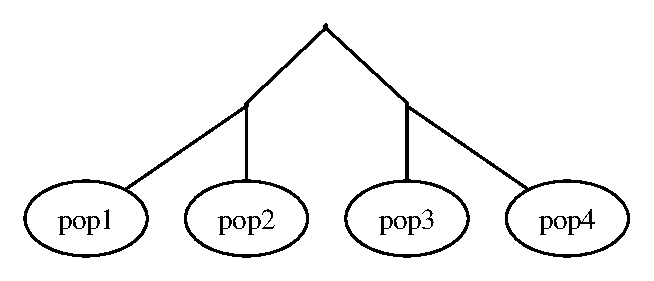
\includegraphics[width=15cm]{f4-phylogeny.eps}
  \end{center}
  \caption{Hypothetical phylogeny for four populations. If you're
    wondering why it's upside down, I warned you. Population
    geneticists look at the world backward from other people. It's
    conventional to draw phylogenies this way in population genetics,
    probably because, being geneticists, population geneticists tend
    to think of them as pedigrees.}\label{fig:f4-phylogeny}

\end{figure}

We can also define
\[
  f_3(1,2,3) = (p_1 - p_2)(p_1 - p_3) - \frac{p_1(1 - p_1)}{n_1} \quad ,
\]
where $n_1$ is the sample size in population 1. The extra term,
$\frac{p_1(1 - p_1)}{n_1}$ makes $f_3$ an unbiased estimator. $f_3$
measures how much common history $p_2$ and $p_3$ share that is
independent of $p_1$. If the true population phylogeny looks like the
one in Figure~\ref{fig:f3-phylogeny}, then
\begin{eqnarray*}
  \mbox{E}\left(f_3(1,2,3)\right) &>& \mbox{E}\left(f_3(2,1,3)\right) \\
  \mbox{E}\left(f_3(1,2,3)\right) &>& \mbox{E}\left(f_3(3,1,2)\right)
  \quad . \\
\end{eqnarray*}
Finally we can define
\[
  f_2(1,2) = (p_1 - p_2)^2 - \frac{p_1(1 - p_1)}{n_1} - \frac{p_1(1 -
    p_1)}{n_1} \quad ,
\]
which gives an unbiased estimate of squared allele frequency
differences between populations, analogous to pairwise
$F$-statistics. 

\begin{figure}
  \begin{center}
    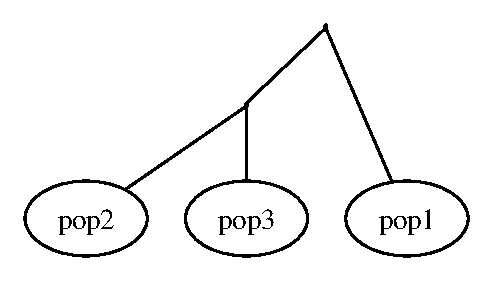
\includegraphics[width=15cm]{f3-phylogeny.eps}
  \end{center}
  \caption{Hypothetical phylogeny for three populations.}\label{fig:f3-phylogeny}
\end{figure}

\bibliography{popgen}
\bibliographystyle{plain}

\ccLicense

\end{document}
